\documentclass{article}
\usepackage{float}
\usepackage[export]{adjustbox}
\title{ABOVE Server Documentation \\ Version 1}
\date{\today}
\author{Casey Daniel}

\begin{document}
\maketitle
\newpage 
\tableofcontents
\newpage
\section{Introduction}

This documentation is meant to be a user guide for the ABOVE server files. These files include the TCP server, Initial Ingestion, plot generation, and shell scripts. All source files can be found on the server on /data/vlf/src/, however this may change on the new server once set up. 


\section{Directory Tree}

Table 1 provides a summary of the relevant directories and information on where to find certain files.

\begin{table}[H]
\begin{tabular}{|c|c|} 
\hline
root & $/data/vlf/$ \\ \hline 
source directory & $/data/vlf/src$ \\ \hline
raw data & $/data/vlf/RawData$ \\ \hline
malformed files & $/data/vlf/malformedFiles$ \\ \hline
data tree & $Year/Month/Day/Site/Hour$ \\ \hline
chunk files & $/data/vlf/chunks/data tree$ \\ \hline
full data files & $/data/vlf/full\_ files$ \\ \hline
logs & $/data/vlf/logs$ \\ \hline
summary plots & $/data/vlf/summaryPlots/data tree$ \\ \hline
\end{tabular}
\label{table:directories}
\caption{Directory List}
\end{table}

\section{TCP Sever}
The Python TCP server it's self is written in Python 2.7, and is needed to run. In the source directory the server is managed by the executable of the form source $directory/tcp\_ server/tcp\_ server\_ PORTNO.py$ where PORTNO is the desired port number. This executable looks for one of 3 commands, start, stop, or restart. (i.e. $./tcp\_ server\_ 26000.py$ start)

If another port is desired a few changes need to be made to the python file. The file needs to be renamed with the new port number, and near the top of the file, the variable $PORT\_ NUMBER$ changed to match.

The server flow is described in figure \ref{fig:serverFlow}, once I finish making it. This will detail the communications flow between the client on the FPGA and the server. 

\begin{figure}
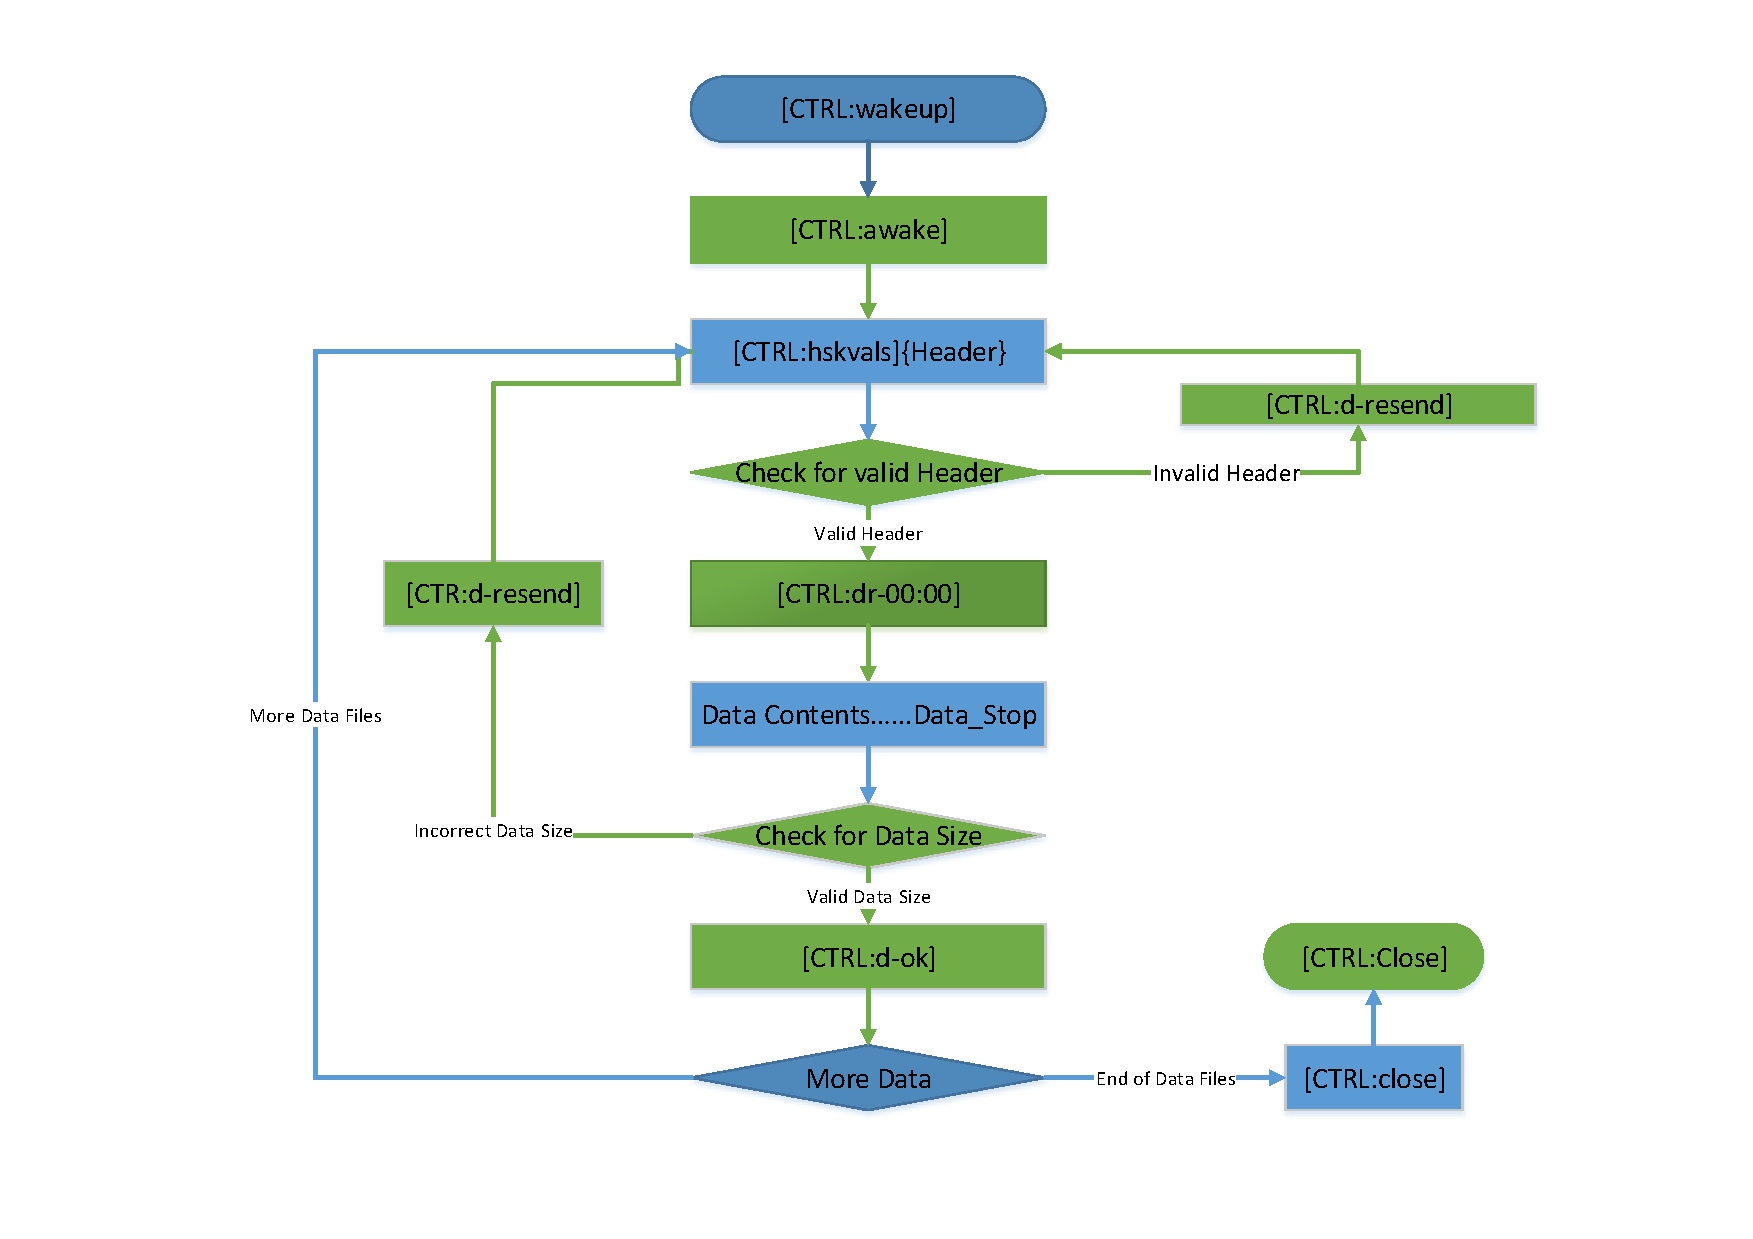
\includegraphics[width=1.5\textwidth,left]{./SeverFlowChart.pdf}
\caption{Visual of the connection process. Blue represents information sent by the client, and green represents information or decisions made by the server.}
\label{fig:serverFlow}
\end{figure}


The client will send over chunk files over the internet connection, and will deposit them in the raw data directory. 
\section{File Manager}

The File Manager, as found in ingestion software directory, and is responsible for file management. It runs the same way the tcp server does, and the same commands and format are used. This file looks through the rawData directory and collects the chunk files produced by the server and combines them into a full file, and deposit in the full file tree.

The File Manager is run on a damon script. When the \texttt{clean\_ up()} method is called, a search of the raw data directory is done. A check for a set of data files is done. If a set contains the expected number of files, as set in the header of the files, they are combined and a full file is saved in the full file directory, and the chunks are then moved to the chunks directory. 

If a full set of files is not found, and the time stamp is over one hour old, then the chunk files that are found are then moved to the malformed files directory. File Manager is also responsible for sending RTEMP Information. These packets are formed and sent from this script, for information on format please contact Darren Chaddock.

After the files are formed, Eric Davis' script for the phase data is then started in a separate thread. Once the clean up is complete, a timer is set for 5 minutes for clean up to be called again.


\section{Summary Plot Generation}

Summary plot generation is handled by Matlab scripts. There are four scripts that handle the summary plots and the availability plots, two for each. One of these is called by a cronjob periodically (see the appendix) and will only search through the previous and current days directories, while the other meant to run on its own and search through the entire directory tree. The summary plot files are \texttt{plot\_ maker.m} to be called by the cronjob and \texttt{full\_ plot\_ maker.m} regenerates all missing summary plots. Similarly availabilityPlotter.m is called by the cronjob and fullAvailabilityPlotter.m is meant to regenerate all of the availability plots.  

The crontab calls a shell script stored in src/shellScripts/. The shell scripts then call the Matlab scripts. 

All of these can be run from the command line using the command 'Matlab -nodesktop -nodsiplay -r run "/path/to/script/scriptname.m"'. It's recommended that when running the regeneration scripts that you move the other Matlab scripts out of the directory to ensure they are not run. Matlab is a resource hog, and leaving these scripts in place can cause a bottle neck on the CPU. There is also a shell script regenerations.sh in src/shellScrips/ directory that will manage these scripts. 

\section{SD reader}

The SD reader application is a c++ script that will read the contents of the SD card, and place them in the directory tree with a given root directory. To run this program in the command line "./sdCard if=/path/to/InputFile.dat od=/root/of/directory/tree". There are also 2 optional commands. -hf will fix the header values. The early versions of the SD card had a few fields with incorrect information. -sd \texttt{SD\_ SIZE} will allow you to change the SD card size. The default is 128GB, however if the card is a different size, then a different one can be use. It's recommended to direct the output to a log file by attaching ">log.txt" to the end of the command. 

Before running, the SD card should be copied into a separate file. The mounting point for the SD on a unix system can be found by looking through /dev/ using diskutil. Once the mount point is found, the command dd 1f=/path/ of=out/file.dat can be used to transfer the documents. The /out/file.dat can then be fed into the SD reader. 

\section{FTP Server}
The FTP server is handled by VSFTPD, and can be started by the su by running the command \texttt{"vsftpd /etc/vsftpd/above\_vsftpd.conf"}. This opens an anonymous FTP server with the the summary plot directory as root. At a later time this will also include CDF files. These allow the summary plot page to view the the plots on the web.


\section{Shell Scripts}

There are a few shell scripts. These primarily handle the generation of summary plots. There is also a reboot script that is called by the crontab on boot to restart the server and the file manger. There is also a \texttt{root\_reboot} shell script that is called by the root user on boot to start the FTP server. 

Note: on the current server the reboot scripts don't work and need to be run by hand when the server is rebooted, however with the new server hardware it should be functional.

\section{HTML Page}
In the summary plots page directory sit a simple HTML page to be able to view the summary plots from the browser. It consists of a simple form with the year, month, day, year, hour, site, and a few buttons to be able to flip through both the availability charts and the summary plots.

The year is not automatically generated, and every year the year needs to be added to the form. 

Below the form is the java script that will react to the buttons and pull up the requested image from the FTP server, and display an error message if they are not available.


\section{Installation}

To install the server software on a new server, all the files should be placed in a source directory. All the directories in the directory table should be worked out on the new server, and updated in any python and Matlab script. These directories are commonly named and labeled near the top of the files.

Ensure both python and Matlab are installed. The python packages numpy, scipy, and matplotlib also need to be installed.

The TCP server should be started on the desired ports, and the sites can be remotely configured with the updated ports and IP addresses. Following which the file manager should be started.

Cronjob's calling the shell scripts should be set up. It's recommended that the availability plots and the summary plots generation script be timed so they are called at different times to prevent Matlab becoming a huge resource hog. The current set up can be seen in the crontab section, however this can be tailored as desired.

The HTML page also needs to be updated with the new IP address. It's listed as a constant in the java script. The site is currently hosted by Darren Chaddock, and the new HTML page should be sent to him to be updated. 

\subsection{Crontab}
Here is the current crontab setup to be used as an example. For more options on crontab, please consult their documentation.

Main User Crontab

\texttt{1,30,50 * * * * /data/vlf/src/shellScripts/matlabSummaryPlot.sh \&> /data/vlf/logs/plottingscript.log}

\texttt{@reboot  /data/vlf/src/shellScripts/reboot.sh \&>/dev/null}

\texttt{15,45 * * * * /data/vlf/src/shellScripts/matlabAvailabilityPlotter.sh \&> /data/vlf/logs/avail\_log.log}

Root Crontab

\texttt{reboot /data/vlf/src/shellScripts/root\_reboot.sh \&> /dev/null}

If you wish to see the output of these scripts, the file can be adjusted.



\end{document}